%----------------------------------------------------------------------------------------
%----------------------------------------------------------------------------------------
%----------------------------------------------------------------------------------------
%Method
%----------------------------------------------------------------------------------------
%----------------------------------------------------------------------------------------
%----------------------------------------------------------------------------------------

\section{METHOD}
\label{sec: method}
 \subsection{Self Organizing Maps}
 \label{sec: som}
 
 Kohonen Self organizing map (or self organizing map, SOM) is an unsupervised neural network for mapping and visualizing a complex and non linear high dimension data introduced by~\citep{Kohonen82}. 
 The SOM is a technique that shows a simple geometry relationship of a non-linear high dimension data on a map \citep{Kohonen98}.
 The SOM is a clustering method which reduces the dimension of data to lower dimensions usually 1 or 2D while preserving topological features of the original data.
 Results of SOM contains nodes (usually hexagonal ones) that arranged in 1D or 2D arrays.
 
  
 Each nodes may contain one or more samples from input data and distance between nodes represents similarity or dissimilarity of underlying samples. 
 In the way that similar data are closer together in the array and the further nodes go from each other, the more dissimilarity appears between their samples.
 %Sahar_self_notes: maybe "some" is better instead of one or more
 Moreover,a weight vector ``\boldit{W}" with same dimension of the input data associates with each node which will be change during the process and has a key factor in a position of nodes in the map. 
 
 \cite{Geach12} presented the application of the SOM and demonstrate the algorithm of the SOM in detail. In this section we are going to talk briefly about the algorithm of the SOM, how we create our maps and a test model which will help to interpret our results. %PB20160218: contrast SOM with principal component analysis (PCA), which may be more familiar?
 
 \subsubsection{Algorithm of SOM} 
 \label{sec: algorithm}
     Assuming we have a data set which contains vectors, \boldit{V} $\in \Re^n$ and we want to map them on S1 by S2 map. 
     We start by creating S1 $\times$ S2 empty neurons. 
     The initial arrangement of these neurons depends on a map's topology provided by user.
     Since the topology of the map does not have any affect on the final result, we chose hexagonal topology which is the default topology for SOMs.
     Then, we assign a random weight vector \boldit{W} $\in \Re^n$ to each node.
     The process of creating SOM, happens over series of $N$ iterations. 
     During each iteration the weight vectors might change according to the Kohonen learning rule (equation~\ref{equ: weight adj}). 
      In each iteration:
     \begin{enumerate}
        \item Choose a random vector from our data set.
        \item Calculate the euclidean distance for each node j as  $D_j^2= \sum_{i=0}^{i=n} (V_i - W_i)^2$, and find a neuron with ``$D_{j_{min}}$". This neuron is the winner node and is calling Best Matching Unit (BMU). 
        \item  Compute the radius of the neighbourhood of the BMU to find nodes within this radius. The weight vectors of these nodes will be affected in the next steps. This value is arbitrary and initially can be set to be as high as half of the SOM size and then it decades exponentially over each iteration:
        \begin{equation}
            r^t_{BMU} = r^0_{BMU}e^{(-t/\tau)}
        \end{equation}
        where $\tau$ is a decay constant and usually set to be the same as number of iterations, $N$. $r^0_{BMU}$ and $r^t_{BMU}$ is the radius of the neighbourhood at 0th and $t$th iteration, respectively. 
        \item Change the weight vectors of the BMU and all the nodes within r(t) as:
        \begin{equation}
            \label{equ: weight adj}
            w(t+1)=w(t)+L(t) \times R(t) \times(v(t)-w(t))
        \end{equation}
        where $L(t) = L_0 e^{(-t/\tau)}$ is the learning factor which prevents divergence of the SOM and $R(t)=exp(-\frac{D_j^2}{2r^t_{BMU}})$ is the influence rate. $R(t)$ determines how weight of nodes in the neighbourhood of BMU will change.
        \item  Repeat these steps for $N$ times.
     \end{enumerate}
   
     In order to create SOM, we used {\tiny MATLAB} neural network toolbox~\citep[NNT,][]{matlabtolbox}.
     Although size of the SOM could be anything \cite{Vesanto05} suggested that the total number of  $5\sqrt{n}$ neurons provides the most sufficient size.
     SOM in {\tiny NNT} works in two phases. 
     Phase one is the ``ordering phase". 
     This phase starts with maximum neighbourhood distance (which is initially provided by user), and initial learning factor of 0.9 which is a default value for the learning factor. 
     The ordering phase continues for requested number of iterations and during that steps changes the parameters in the way that in the last iteration learning factor is 0.02 and the neighbourhood distance is 1.
     
     The second phase is the ``tuning phase".
     In this phase the neighbourhood distance is at its minimum, but learning factor decreases very slowly.
     This minimum neighbourhood distance and slowly decreasing the leaning factor helps to fine tune the topology results and causes the more stable SOM. 
     The number of iterations in this tuning phase most be much more than the number iterations in ordering phase, to allow the tuning happens slowly. 
     We chose number of epochs the tuning phase be 3 times more than number of epochs in the ordering phase.
     
     To show our results, we combine two of the {\tiny NNT}'s built-in plots. 
     A Hits map, which shows number of hits for each neurons, and a distances map, which shows the same neurons and the distance between them. 
     To combine these two maps, we wrote number of hits in each neurons in the neurons in a distance map.
     The neurons with zero hit, left empty  (i.e. Fig~\ref{fig: testmodel2by2}).
     In distance maps, the grey hexagonal shape areas represent the neurons.
     The red lines between neurons, show the immediate neighbours.
     The distances in a distance map are showing by colours.
     The darker colour represents the larger distance between neurons; whilst the lighter colours means there is small distance between neurons.
    
     We created different SOM with different grids, initial neighbourhood, and iteration numbers to find the optimize result for our sample.
     varying grids of the maps helps us to monitor whether grouping regions in smaller maps is real or its because of the shortage of the neurons.
     We test our code by varying the number of iterations in the ordering phase and find $N = 100$  is optimized for our sample.
     In Section~\ref{sec: test model} we used NNT to create SOMs from SED of galaxies and learn how this method works and how we can interpret the results.
   
 \subsection{Test Model}
 \label{sec: test model}
 %the sole puprpes of this section is to show how to read the SOM results. 
    Before we start creating SOM for our data, we apply this model on an already studied sample. 
    Our test sample contains spectral energy distribution (SED) as well as properties such as age, stellar mass and specific star formation rate of 142 galaxies with redshift 0.5 $ \leq$ Z $\leq $ 1, which were measured and studied by \cite{Hossein12}. 
   % \cite{Hossein12} used supervised neural network method to classify galaxies' spectrum based on SED models from \cite{Kinney96} and \cite{Coleman80}.
    We used SOM to group galaxies based on their SED. For each galaxy, fluxes on different wavelengths were an input of the program. % PB20160218: should say how many data points per galaxy. Comment on the individual flux points not being statistically independent? Also, this is a fairly different sort of dataset than the M31 data, so need to explain how applicable.
    
    Then, We created various SOM maps with different girds and neighbourhoods. 
    For each map, SOM grouped the galaxies based on their similarities. 
    Galaxies with the most similarity in their SED gathered in the same neurons, the one with more similar spectral type have a light colour (i.e. bright yellow) between them, and the galaxies with the least similarity in their spectral type have black colour between them (Figs~\ref{fig: testmodel2by2} and~\ref{fig: testmodel3by2}).
    
    To illustrate these results more clearly, we averaged SED of the galaxies in each neurons and showed them in the same order as neurons in SOM (Figs~\ref{fig: sed_testmodel2by2} and~\ref{fig: sed_testmodel3by2}). 
    Figs~\ref{fig: testmodel1} and~\ref{fig: testmodel2}, shows SOM results and the SED corresponding to them in $2\times2$ and $3\times2$ grids, respectively.  
    Top panel of the Fig~\ref{fig: testmodel1} shows the combined hits and distance map for  $2\times2$ map. Since numbers in each neurons is the numbers of the galaxies in that neurons, we can say we divided our 142 galaxies in a group of 30, 50 and two groups of 29. In lower panel of Fig ~\ref{fig: testmodel1}, plot (a) shows averaged SED of 30 galaxies, plot (d) shows the average SED of 50 galaxies, and plots (c) and (b) show the average SED of 29 galaxies. 
    
    The colour between neurons with 34 galaxies and neurons with 54 galaxies is black, which indicate these two neurons have a maximum distance from each other and galaxies in those neurons are the least similar ones. By looking at the average SED plots for those two neurons, one can clearly see that the averaged SED of these two groups of galaxies are completely different. %should I talked about what kind of SED are they. %PB: yes.
    On the other hand, the colour between neurons with 54 galaxies and 29 galaxies is yellow, which shows the similarity and closeness of galaxies in these two neurons. 
    Again, by looking at the average SED plots (c and d), it is clear that the averaged SED of these two groups are the most similar ones. 
    In Fig~\ref{fig: sed_testmodel2by2} plots (a) and (b) shows some similarity, if we look at the distance map (Fig~\ref{fig: testmodel2by2}) we could see colours between neurons related to these two groups is bright orange which is relatively bright which represents some similarity between these two groups.
    
    In Fig~\ref{fig: testmodel2}, although the number of galaxies in each neurons are smaller due to higher number of neurons, one could see similar patterns. 
    The average SED of the galaxies in neurons connected with bright colours are more similar to each other than the average SED of the galaxies in neurons connected with dark colours.
    In the $3\times2$ grid, since the galaxies have more space to separate, they gathered in the smaller groups. 
    However, most of the galaxies, which shared the same neurons, or were in the neurons close to each other, in Fig~\ref{fig: testmodel1} stayed in the neurons which are close to each other.
    
    One can increase the grids of the maps to the point that each neurons contain max 1 galaxy. 
    This situation eventually happens because no two galaxies are exactly alike.
    Even in this case, galaxies with similar SED stay in a area which all the neurons are connected with yellow colour, and the galaxies with different type of SED are separated from them with darker colours (Fig~\ref{fig: testmodel3}). 
    Note that, empty neurons in the SOM results have their weight vectors and if we apply this network on the other set of data, based on similarity of the new data set to our sample, they could sit in the empty neurons.
    %PB20160218: need some additional interpretation of the results
    \begin{figure}
        \centering
        \begin{subfigure}[b]{0.5\textwidth}
            \centering
            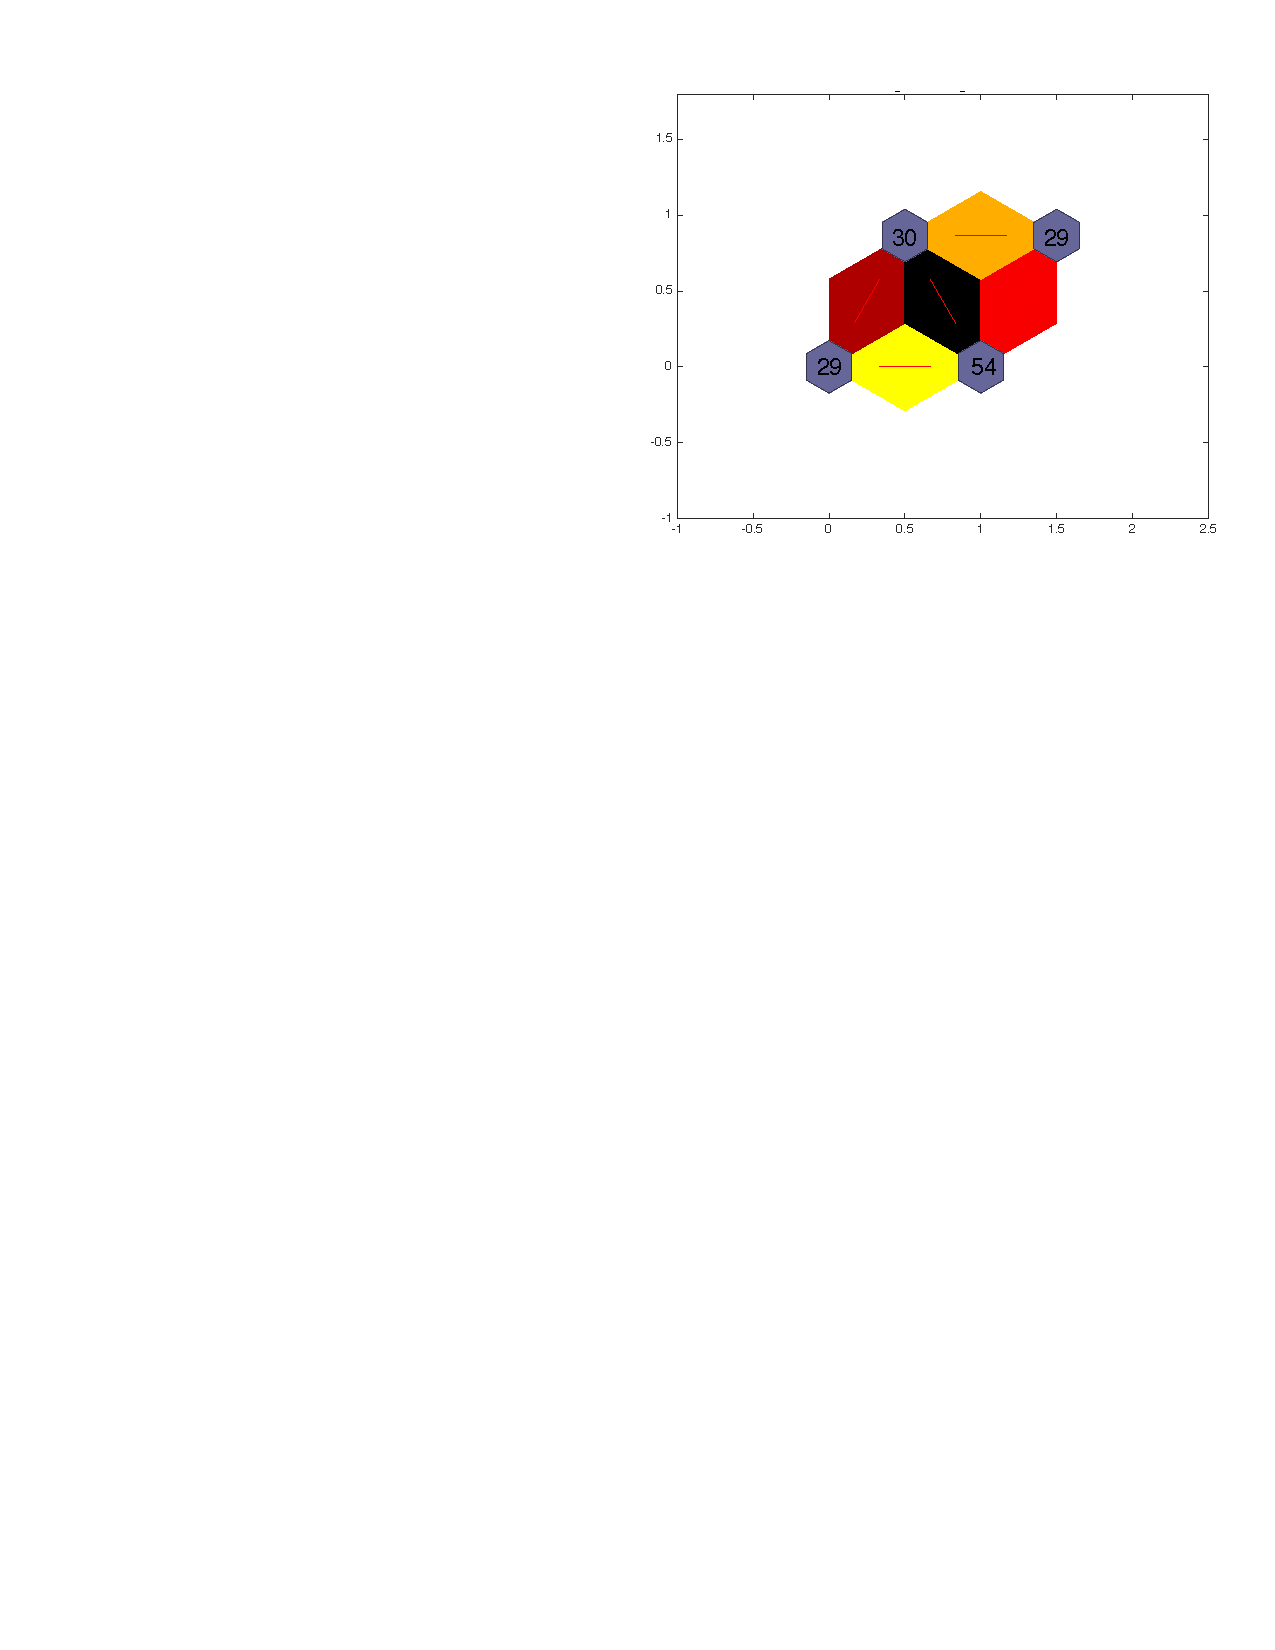
\includegraphics[width=0.7\textwidth]{../images/test_model/2by2_nei3.pdf}
            \caption{A combination of the hits and distance map in $2\times2$ SOM. }
             \label{fig: testmodel2by2}
        \end{subfigure}
        \hfill
        \begin{subfigure}[b]{0.5\textwidth} 
            \centering
            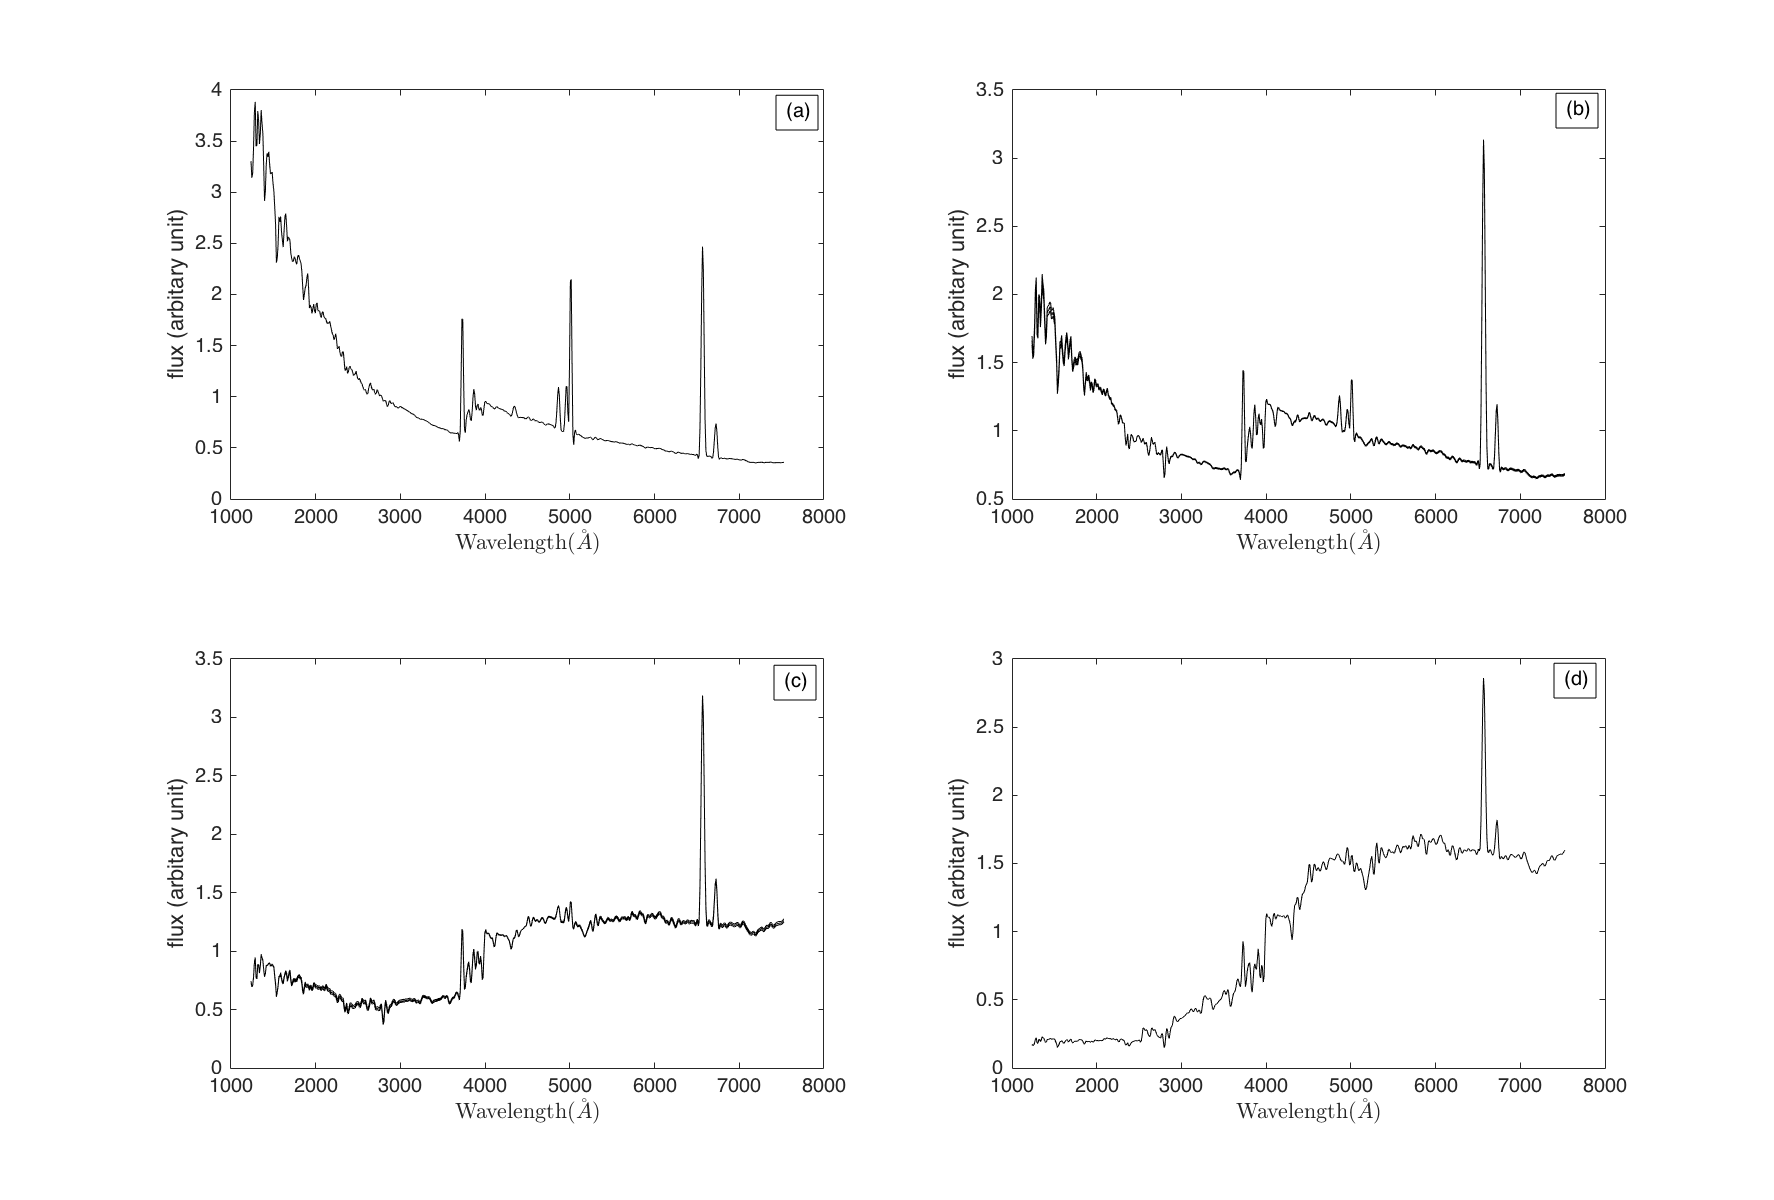
\includegraphics[width=\textwidth]{../images/test_model/SED_total2by2nei3.png}
            \caption{An average SED of galaxies in  $2\times2$ gird.}
             \label{fig: sed_testmodel2by2}
        \end{subfigure}
        \caption{SOM result of the SED of the 142 galaxies in redshift of 0.5 $ \leq$ Z $\leq $ 1 with size of $2\times2$. Top: shows a combination of the hits and distance map in $2\times2$ SOM. Gray hexagonal shape areas represent neurons. Number of on each neurons shows the number of galaxies grouped in that neurons. Red lines connected neighbour neurons to each other, and colours between neurons are a scale of distance between neurons. Bottom: shows the Average SED of the galaxies in same neurons. Plots a, b, c, and d are averaged SED of galaxies in neurons with a number of 30, 29, 29, and 54, respectively.}
        \label{fig: testmodel1}
            
    \end{figure}
    
    \begin{figure}
        \centering
        \begin{subfigure}[b]{0.5\textwidth}
            \centering
            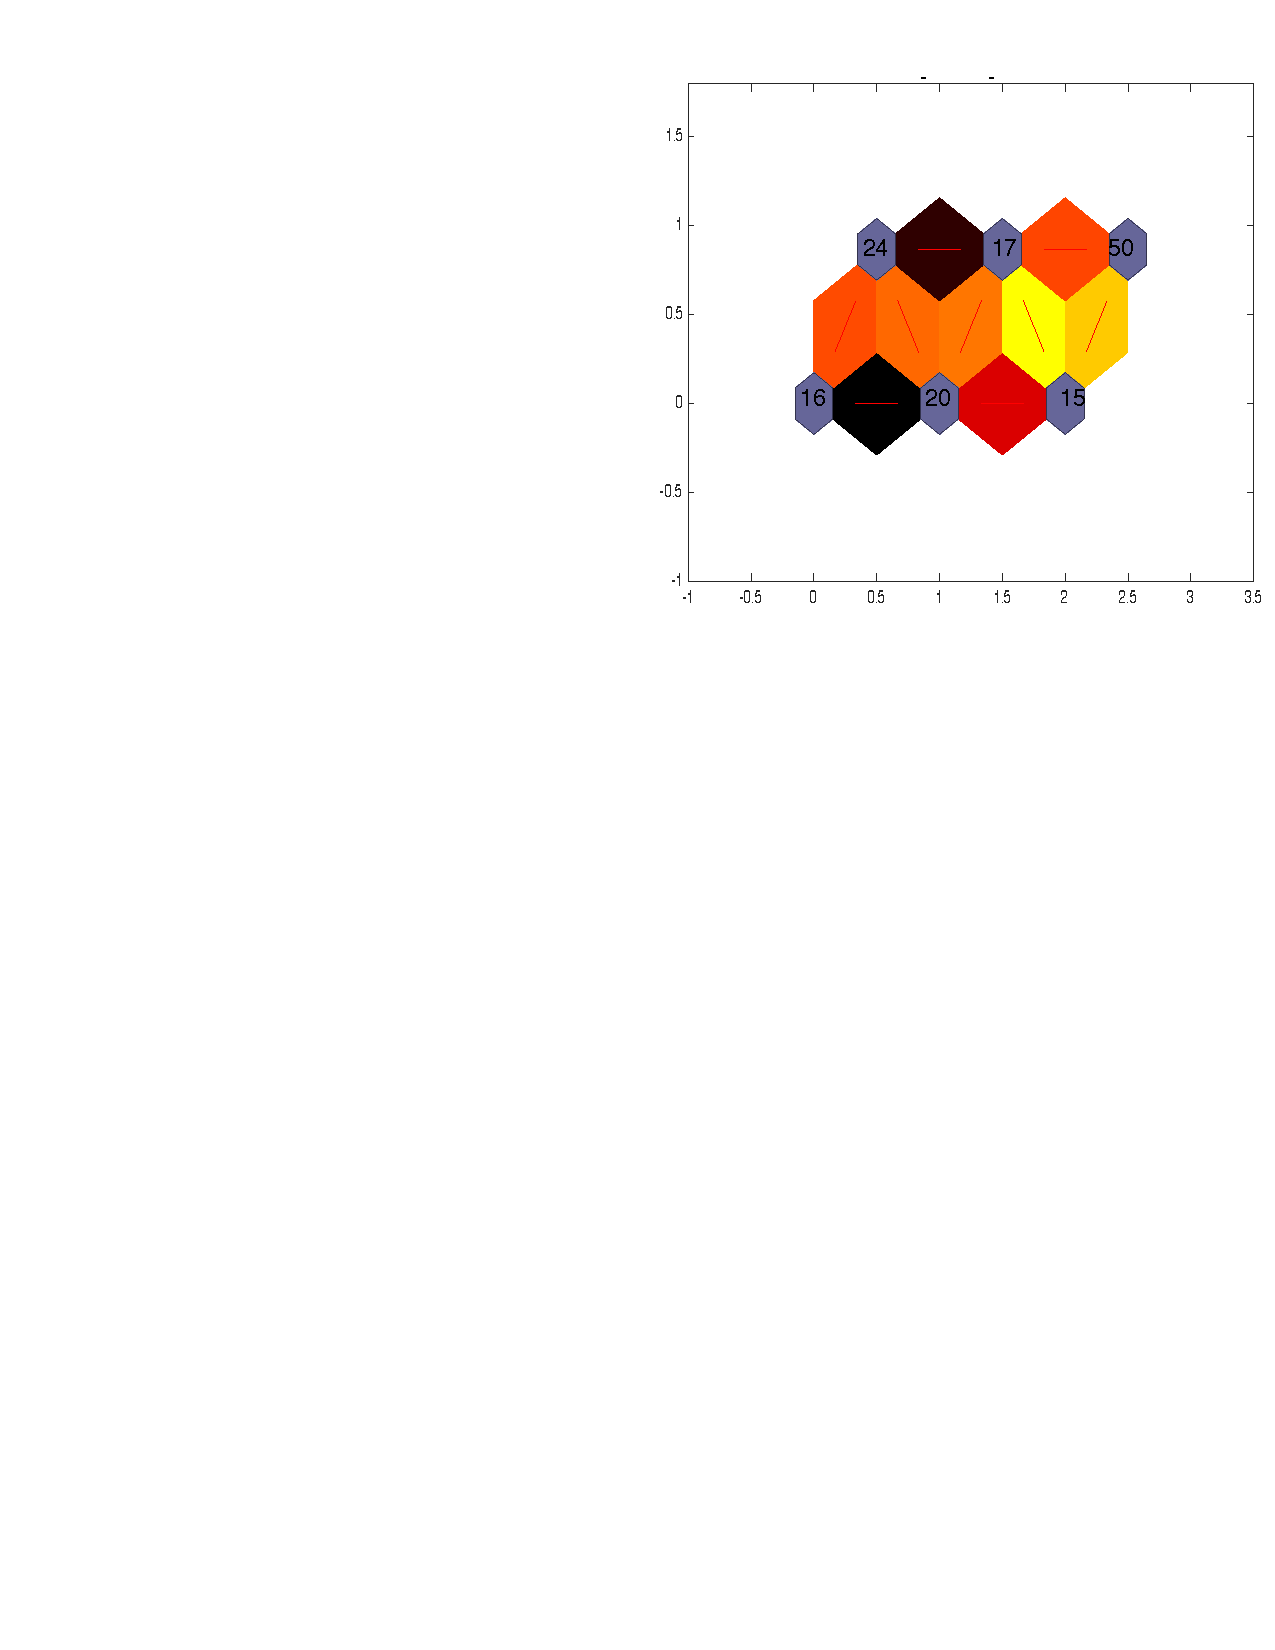
\includegraphics[width=0.7\textwidth]{../images/test_model/3by2_nei3.pdf}
            \caption{The same as Fig~\ref{fig: testmodel2by2} with size of $3\times2$.}
             \label{fig: testmodel3by2}
        \end{subfigure}
        \hfill
        \begin{subfigure}[b]{0.5\textwidth} 
            \centering
            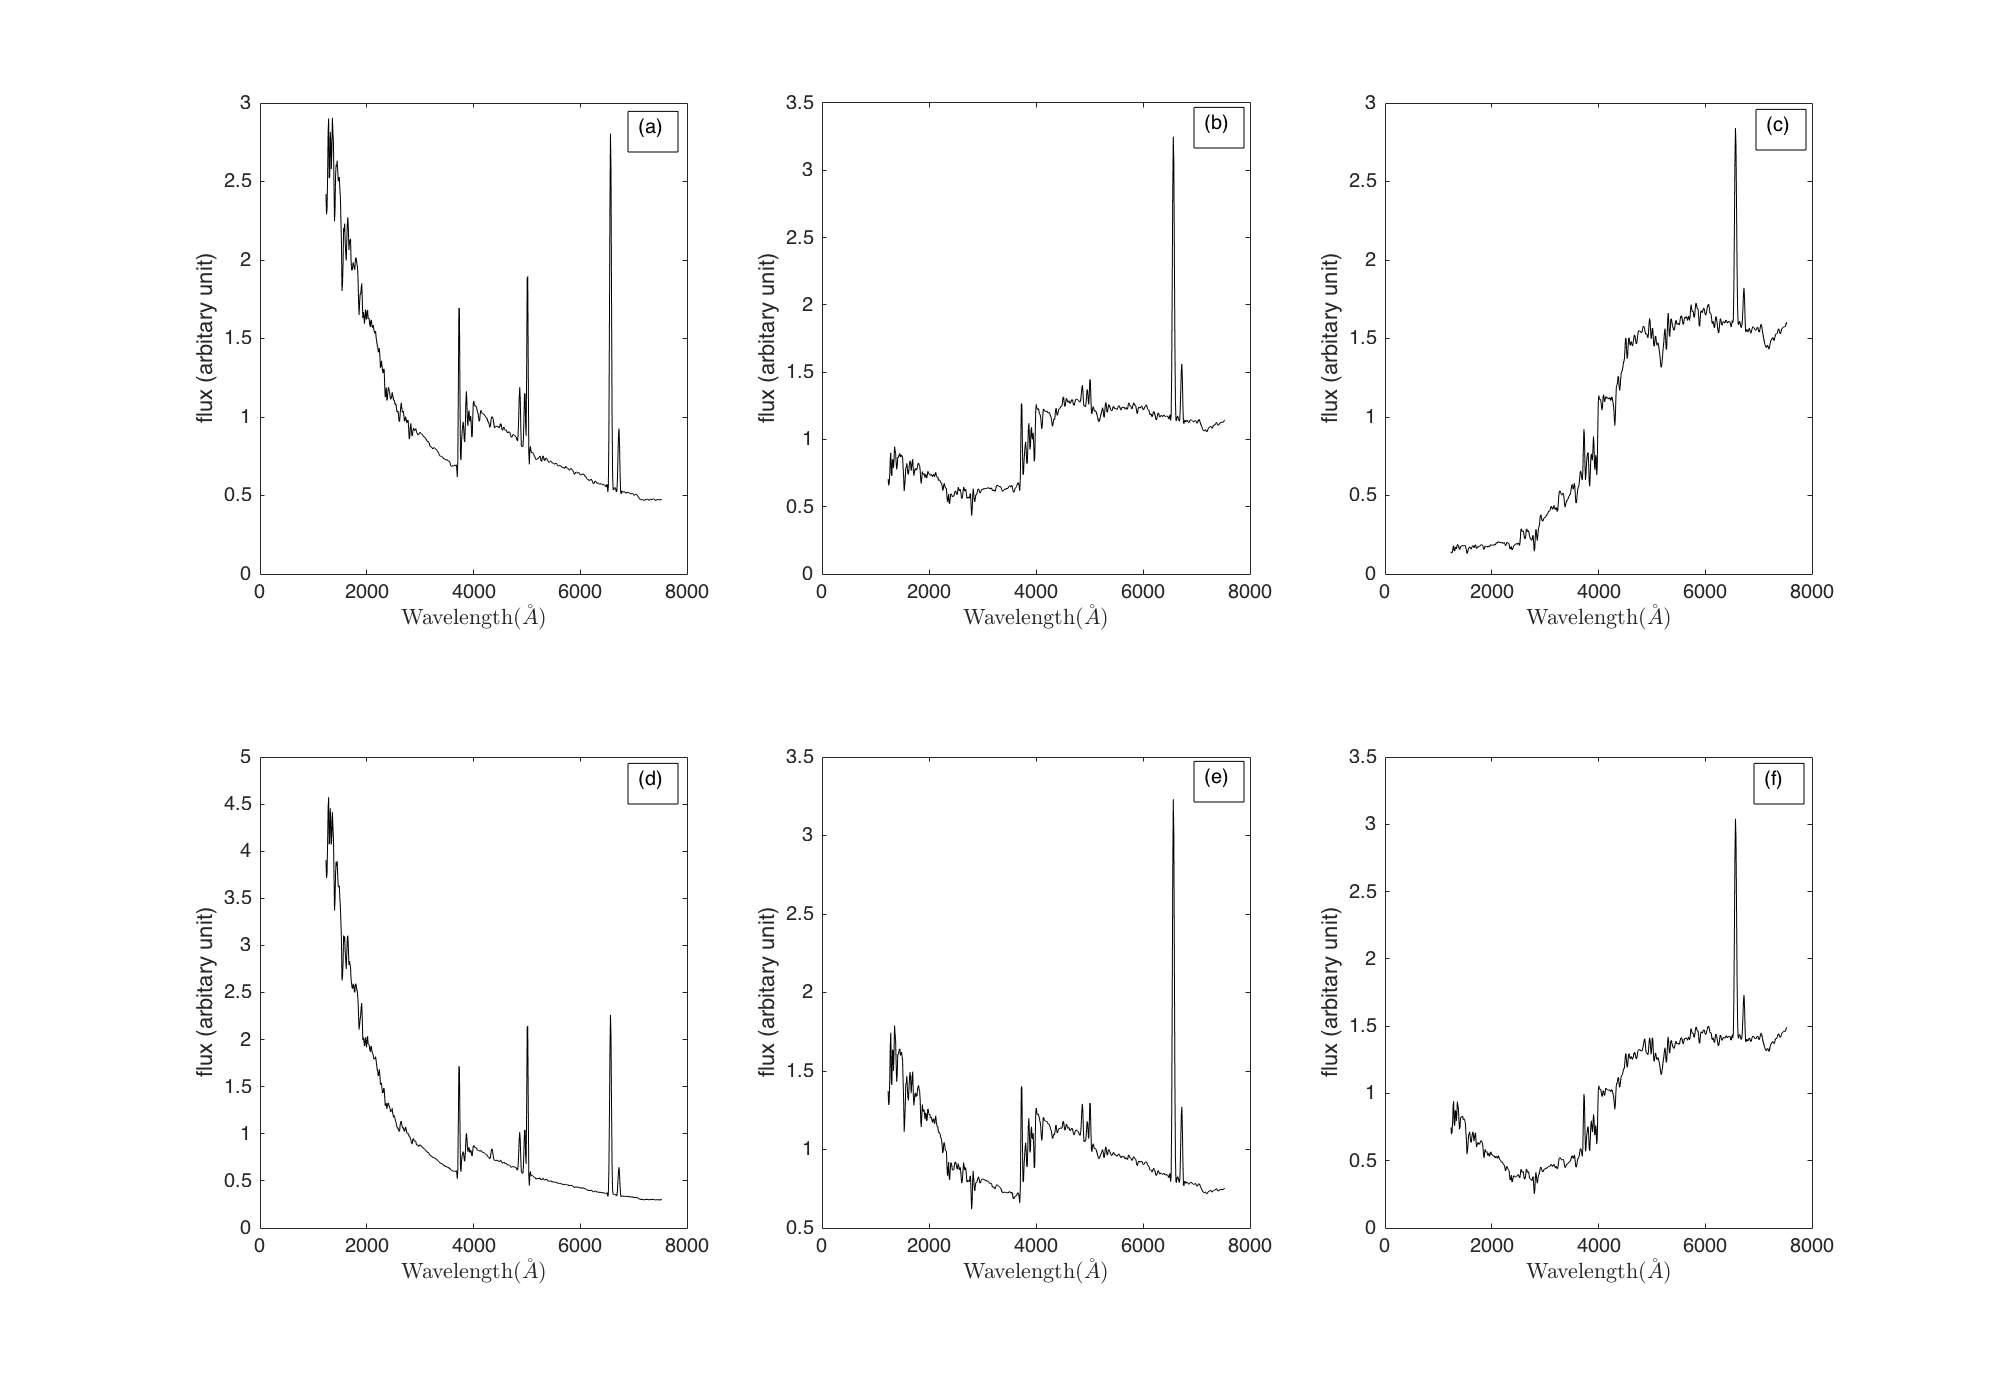
\includegraphics[width=\textwidth]{../images/test_model/SED_total2by3nei3.png}
            \caption{The same as Fig~\ref{fig: sed_testmodel2by2} with size of $3\times2$.}
             \label{fig: sed_testmodel3by2}
        \end{subfigure}
        \caption{The same as Fig~\ref{fig: testmodel1}, but here we show results of SOM with size of $3\times2$.  }
        \label{fig: testmodel2}
            
    \end{figure}
    \begin{figure}
        \centering
        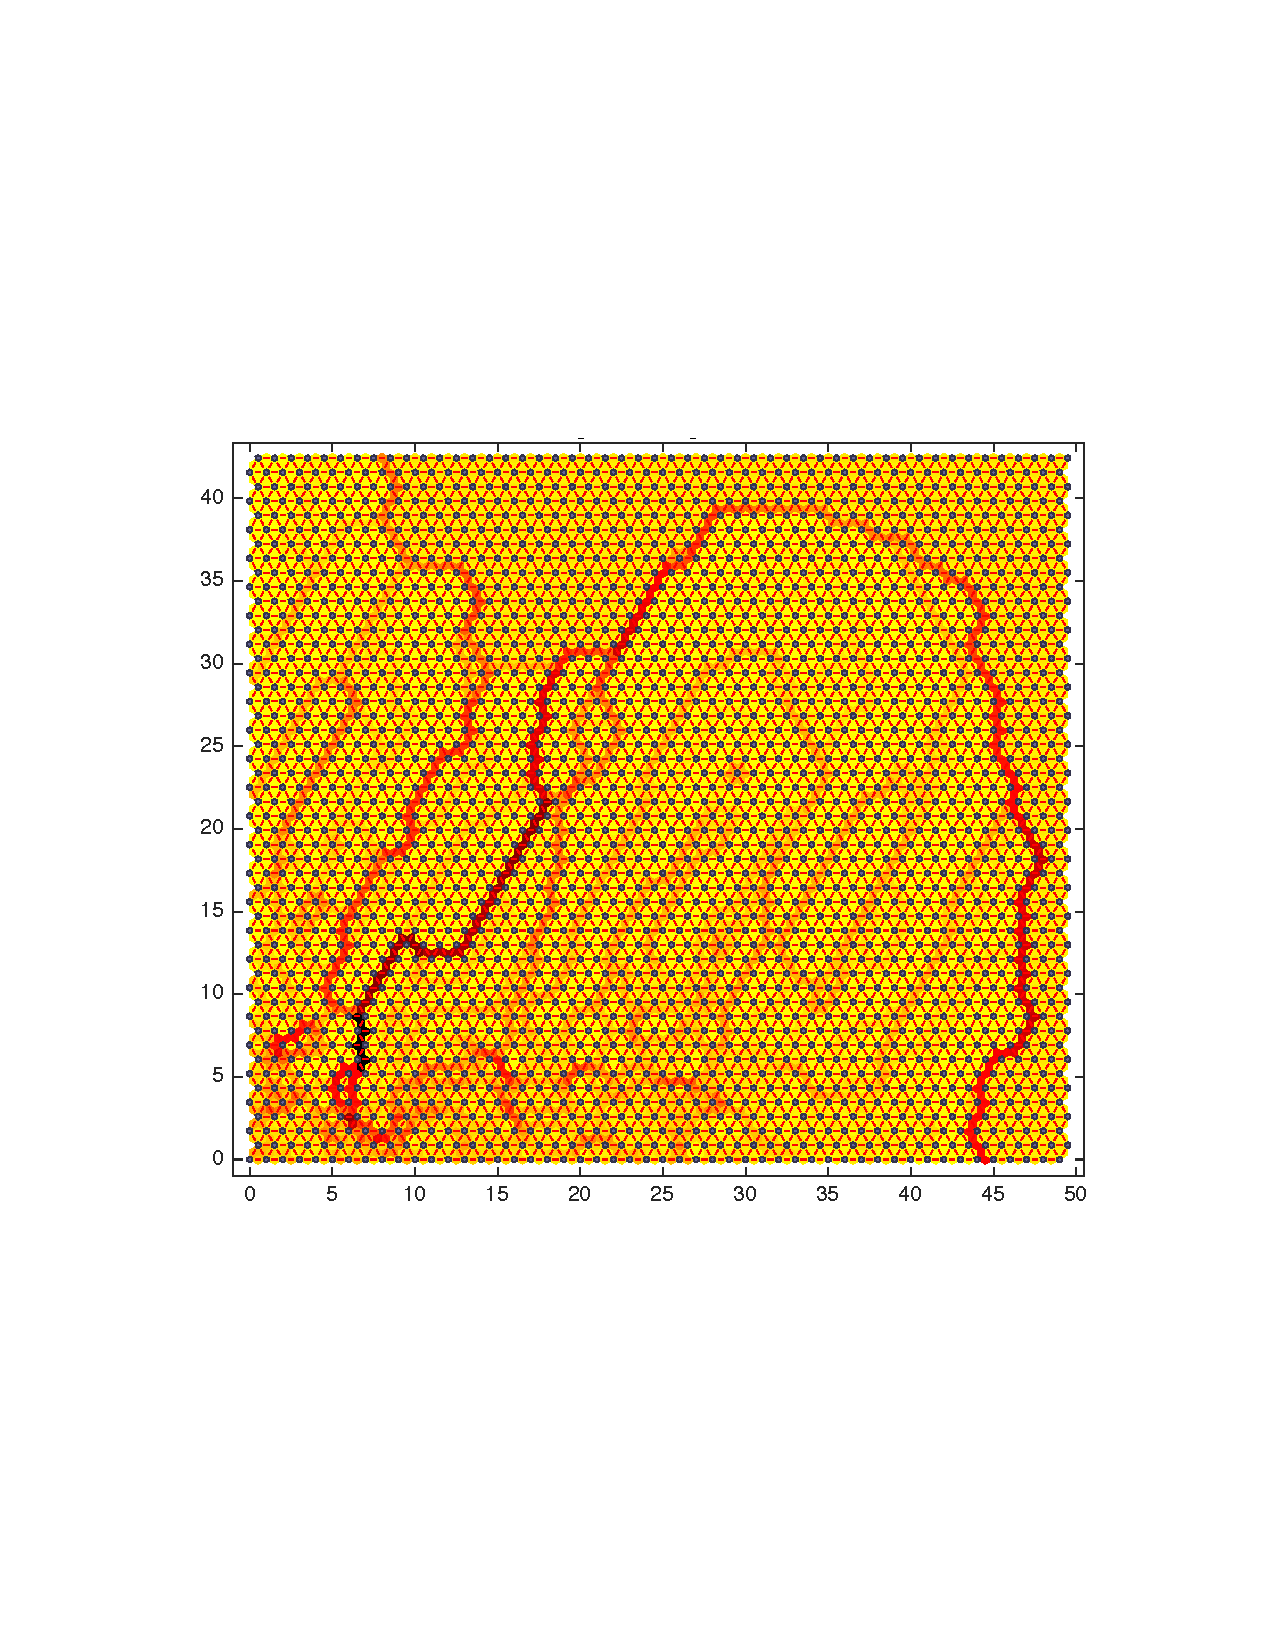
\includegraphics[width=0.4\textwidth]{../images/test_model/50by50_nei3.pdf}
        \caption{The same as Fig~\ref{fig: testmodel2by2} with size of $50\times50$.}
        \label{fig: testmodel3}
    \end{figure}